\documentclass[reqno, 12pt]{article}
\usepackage{amsmath}
\usepackage{amsfonts}
\usepackage{amssymb}
\usepackage{enumerate}
\usepackage{graphicx}
\usepackage{wrapfig}
\usepackage[mathscr]{euscript}
\usepackage{stmaryrd}
\usepackage[normalem]{ulem}
\usepackage{fullpage}
\newcommand{\R}{\mathbb{R}}
\newcommand{\Z}{\mathbb{Z}}
\newcommand{\Q}{\mathbb{Q}}
\newcommand{\N}{\mathbb{N}}
\newcommand{\Lagr}{\mathcal{L}}
\newcommand{\END}{\hspace*{\fill} $\clubsuit$}
\newcommand{\st}{\sout{$\supset$}}
\newcommand{\vx}{ \mathbf{x} }
\newcommand{\vy}{ \mathbf{y} }
\newcommand{\degree}{^\circ}


\title{Functional Analysis Exploration 3}
\author{Zachary Fendler}

\begin{document}
\maketitle
I wanted to learn a little more about Jordan Canonical Forms, at least the basics. I used the Friedberg text and found some confusion in their example. Their example has an eight-by-eight matrix in Jordan Canonical Form and says that $v_7$ is an eigenvector. The issue I have is that the vector has all entries zero which I feel contradicts the definition of an eigenvector. Is there something I am missing/mistaking?
\\\\Section two gives the definition for degree in the regular case. That is
\textbf{Definition 2.1} Let $\Omega \subset \R^n$ be open and bounded. $f \in \bar{C}^1(\Omega)$ and $y \in \R^n\backslash f(\partial\Omega \cup S_f)$. Then we define
$$d(f,\Omega, y) = \sum_{x \in f^{-1}(y)} \text{sgn}J_f(x)$$
where we say $$\sum_{\emptyset} = 0$$ by convention.
Here, $\bar{C}^1(\Omega) = C^1(\Omega) \cap C(\bar{\Omega})$ and $J_f (x) = \text{det}f^{\prime}(x)$ the \textit{Jacobian} of $f$ at $x$.
I tried to draw some examples of what I think the degree functional does.
\begin{figure}[h!]
	\centering
	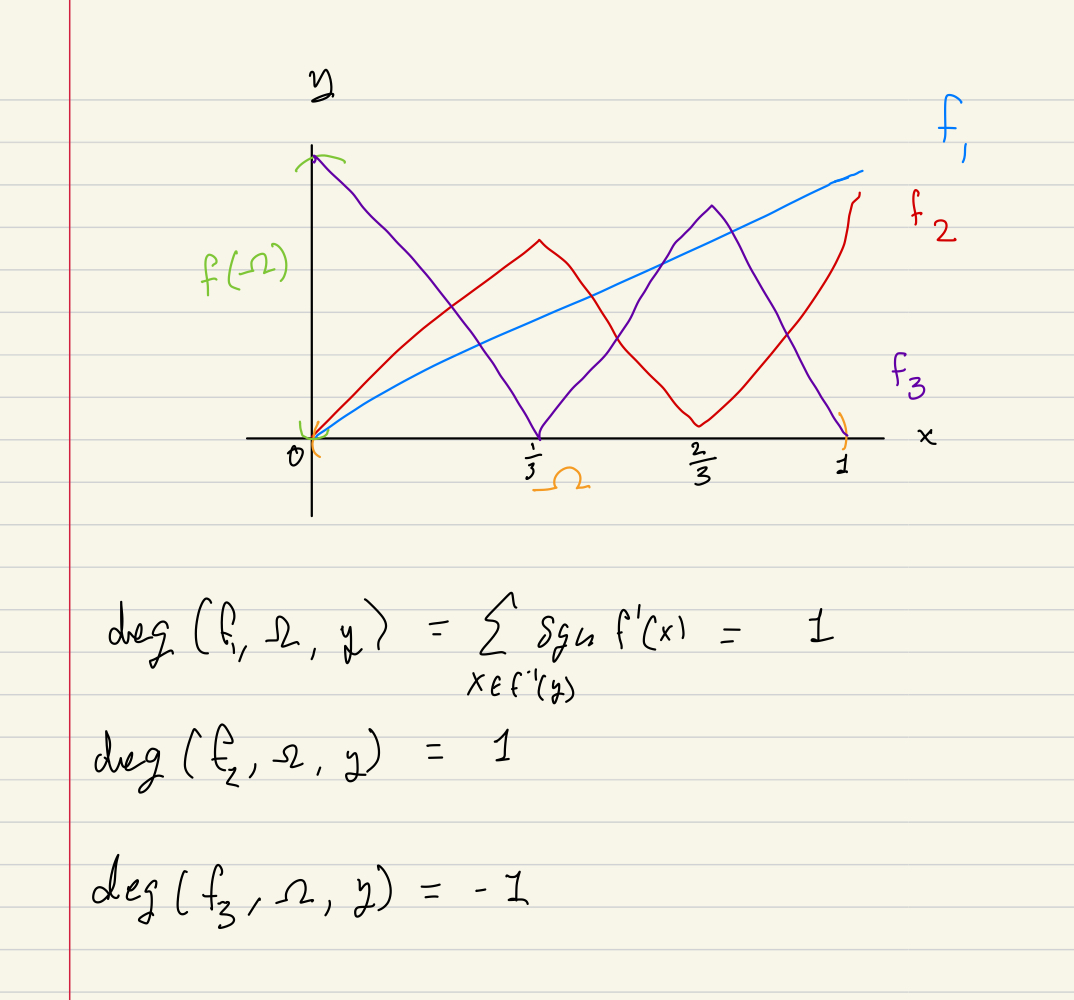
\includegraphics[width = .5\textwidth]{/Users/zacharyfendler/Documents/TeX/images/degree1.jpeg}
	\caption{Illustration of degree in one dimension on the unit interval in the regular case.}
\end{figure}
My current struggle in understanding of the definition of the regular case is the $x \in f^{-1}(y)$ in the summand. It is important to keep in mind that we are currently interested in $f(x) = y$. Then, for example, when $y=0.5$, $f_1$ will only hit $y$ one time and the derivative is positive. So the degree is $1$. This follows for all $y$ on this particular function. Similarly, for $f_2$, if $y=0.5$, $f_2$ likely has $3$ points $x_1,x_2,x_3 \in \Omega$ such that $f_2(x_i) = 0.5$ for $i = 1,2,3$. Suppose $x_1 < x_2 < x_3$ then, according to the illustration, the sign of the derivatives for each point respectively are $+1, - 1, +1$ and summing to $+1$. Some of the proofs in section two I found hard to understand. Particularly, propositions 2.1 and beginning of subsection 2.2. I know my integration understanding is weaker in real analysis but it is the usage of mollifiers that confuses me. Intuitively, I need to remember that mollifier functions are used to be a smooth approximator for a function or functions of interest. I was able to get a picture for subsection 2.2 set up. It is the integral part that is difficult.
\begin{figure}[h!]
	\centering
	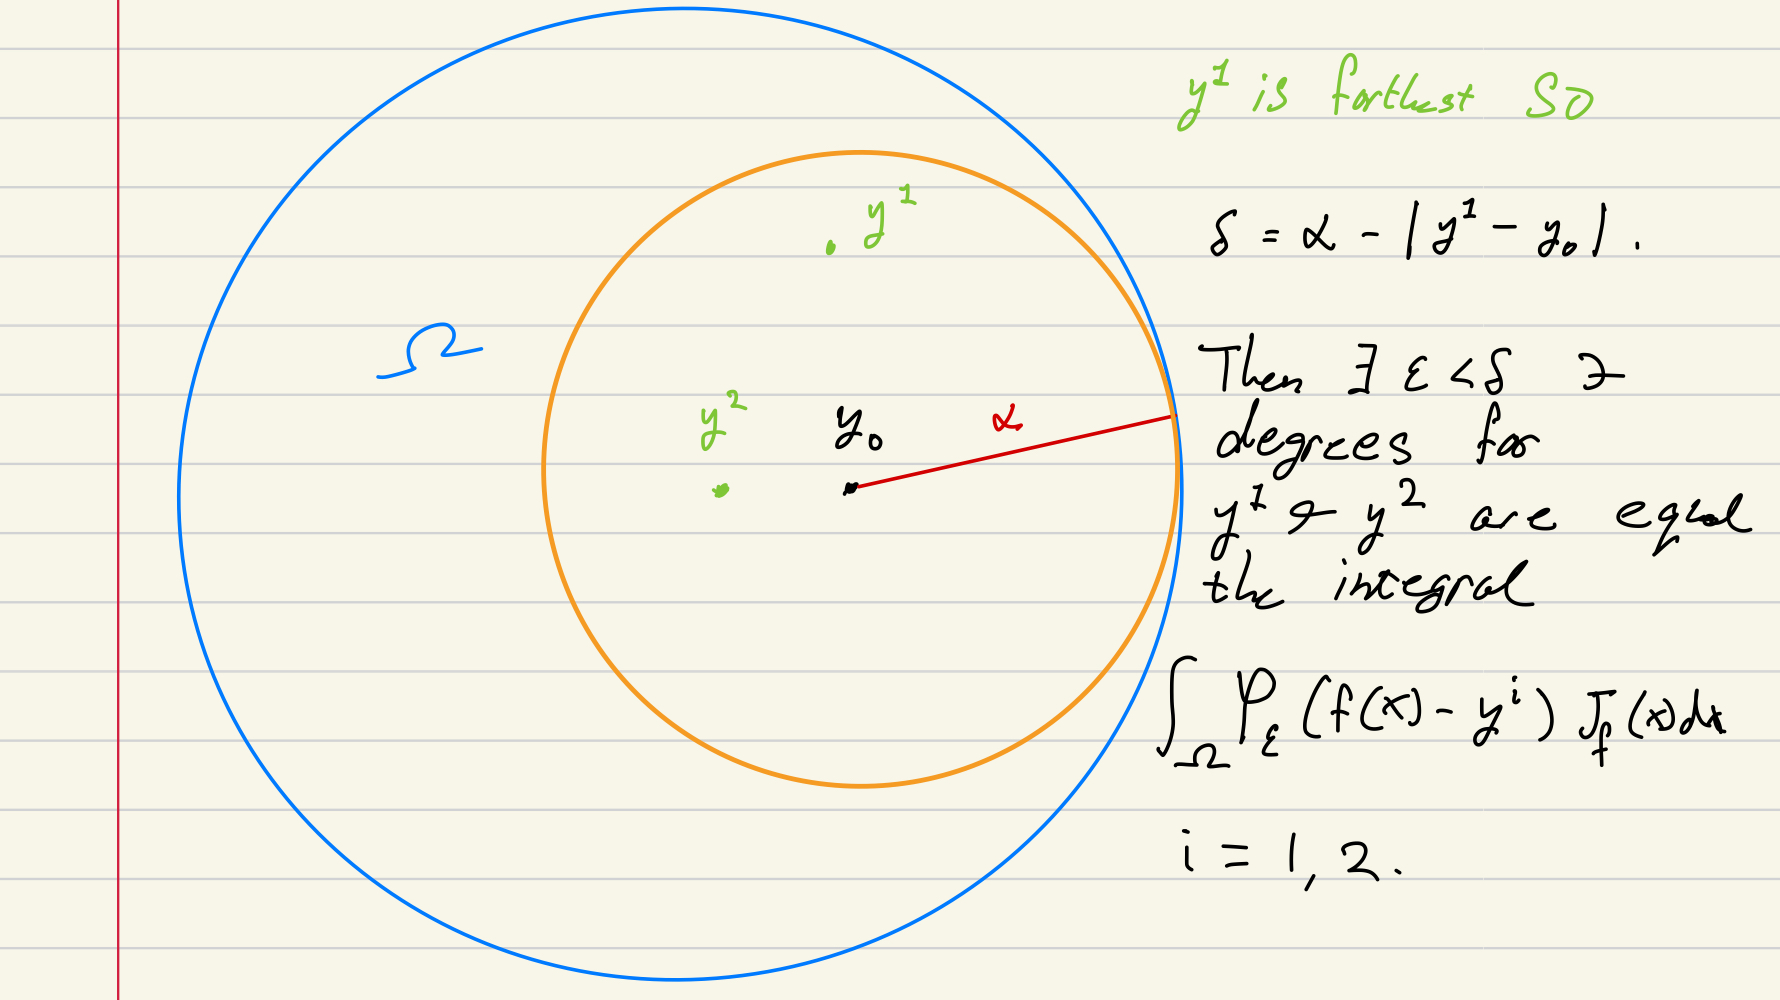
\includegraphics[width = .5\textwidth]{/Users/zacharyfendler/Documents/TeX/images/subsect2-2.jpeg}
	\caption{Example of the set up in Deimling proposition 2.2}
\end{figure}
In words, I believe that proposition 2.1 gives us a new definition for degree in a more general case using the mollifier function. Subsection 2.2 is applying the new definition to allow us to consider singular values. Recall the definition of mollifier as $\varphi_\alpha : \, \R^n \rightarrow \R$ given by 
$$\varphi_1 = \begin{cases}
	c\cdot \text{exp}\left(-\frac{1}{1- |x|^2}\right) \qquad &\text{for} \, |x| < 1 \\
	0 \qquad &\text{otherwise}
\end{cases}$$
where $c > 0$ such that $\int_{\R^n}\varphi_1(x) dx = 1$, and $\varphi_\alpha(x) = \alpha^{-n}\varphi_1(x/\alpha)$. In this section, they use $\varepsilon$ instead. 

I am wondering if there is a typo as \textbf{Definition 2.2} generalizes the degree functional to include singular values but says to use Definition 1.1 which is not in the textbook. On another note, the rest of the chapter loosens the conditions of the function $f$ for the degree functional using the degree of another function $g$ that is "close enough", roughly speaking. Again, this is taking a lot of time for me to think about. There are no images in the textbook so far so it is quite dense. I am looking forward to the next section as some results are discussed including Brouwer's Fixed Point Theorem. I am hoping there will be some images available in the text or elsewhere for the more famous results. \END

\end{document}